\tikzset{every picture/.style={line width=0.75pt}} %set default line width to 0.75pt        

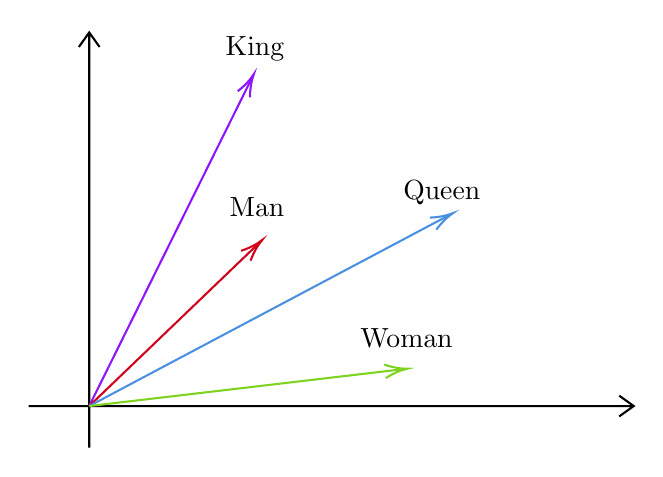
\begin{tikzpicture}[x=0.75pt,y=0.75pt,yscale=-1,xscale=1]
%uncomment if require: \path (0,300); %set diagram left start at 0, and has height of 300

%Shape: Axis 2D [id:dp7833501097464808] 
\draw  (147,218) -- (438.5,218)(176.15,38) -- (176.15,238) (431.5,213) -- (438.5,218) -- (431.5,223) (171.15,45) -- (176.15,38) -- (181.15,45)  ;
%Straight Lines [id:da9722959700270661] 
\draw [color={rgb, 255:red, 144; green, 19; blue, 254 }  ,draw opacity=1 ]   (176.15,218) -- (254.61,59.79) ;
\draw [shift={(255.5,58)}, rotate = 476.38] [color={rgb, 255:red, 144; green, 19; blue, 254 }  ,draw opacity=1 ][line width=0.75]    (10.93,-3.29) .. controls (6.95,-1.4) and (3.31,-0.3) .. (0,0) .. controls (3.31,0.3) and (6.95,1.4) .. (10.93,3.29)   ;

%Straight Lines [id:da1566212605809547] 
\draw [color={rgb, 255:red, 208; green, 2; blue, 27 }  ,draw opacity=1 ]   (176.15,218) -- (258.06,139.38) ;
\draw [shift={(259.5,138)}, rotate = 496.17] [color={rgb, 255:red, 208; green, 2; blue, 27 }  ,draw opacity=1 ][line width=0.75]    (10.93,-3.29) .. controls (6.95,-1.4) and (3.31,-0.3) .. (0,0) .. controls (3.31,0.3) and (6.95,1.4) .. (10.93,3.29)   ;

%Straight Lines [id:da34953036327650255] 
\draw [color={rgb, 255:red, 74; green, 144; blue, 226 }  ,draw opacity=1 ]   (176.15,218) -- (349.73,125.94) ;
\draw [shift={(351.5,125)}, rotate = 512.06] [color={rgb, 255:red, 74; green, 144; blue, 226 }  ,draw opacity=1 ][line width=0.75]    (10.93,-3.29) .. controls (6.95,-1.4) and (3.31,-0.3) .. (0,0) .. controls (3.31,0.3) and (6.95,1.4) .. (10.93,3.29)   ;

%Straight Lines [id:da2649887092664085] 
\draw [color={rgb, 255:red, 126; green, 211; blue, 33 }  ,draw opacity=1 ]   (176.15,218) -- (327.51,200.23) ;
\draw [shift={(329.5,200)}, rotate = 533.31] [color={rgb, 255:red, 126; green, 211; blue, 33 }  ,draw opacity=1 ][line width=0.75]    (10.93,-3.29) .. controls (6.95,-1.4) and (3.31,-0.3) .. (0,0) .. controls (3.31,0.3) and (6.95,1.4) .. (10.93,3.29)   ;


% Text Node
\draw (256,46) node  [align=left] {King};
% Text Node
\draw (257,122) node  [align=left] {Man};
% Text Node
\draw (346,115) node  [align=left] {Queen};
% Text Node
\draw (329,185) node  [align=left] {Woman};


\end{tikzpicture}
